\chapter[The Ketonen-Solovay machinery]{Accessibility inside \texorpdfstring{$\epsilon_0$}{Epsilon0}: The Ketonen-Solovay Machinery\label{ks-chapter}}
\label{chap:ketonen}
\index{maths}{Ordinal numbers!Ketonen-Solovay machinery}

\section{Introduction}
The reader may think that our proof of termination in the previous  chapter requires a lot of mathematical tools and may be too  complex. So, the question is ``is there  any  simpler proof'' ?

In their article~\cite{KP82}, Kirby and Paris show that this result cannot be proved in Peano arithmetic. Their proof uses some knowledge about model theory and non-standard models of Peano arithmetic. In this chapter, we focus on a specific class of proofs of termination of hydra battles: construction of some variant mapping the type \texttt{Hydra} into a given initial  segment of ordinals. Our proof relies only on the Calculus of Inductive Constructions and is a natural complement of the results proven in the previous chapters.

\begin{itemize}
\item There is no variant mapping the type \texttt{Hydra} into the interval $[0,\omega^2)$ (section ~\vref{omega2-case}), and \emph{a fortiori} $[0,\omega)$ (section ~\vref{omega-case}).

\item There exists a variant which maps the type \texttt{Hydra} into the
interval $[0,\epsilon_0)$ (theorem \texttt{every\_battle\_terminates}, in section~\vref{thm:every-battle-terminates}).
\end{itemize}


Thus, a very natural question is the following one:
\begin{quote}
  `` Is there  any variant from
\texttt{Hydra} into some interval $[0,\mu)$, where $\mu<\epsilon_0$, for proving the termination of all hydra battles ?''
\end{quote}

We prove in \coq{} the following result:

\begin{quote}
There is no variant for proving the termination of all hydra battles
from \texttt{Hydra} into the interval $[0..\mu)$, where
$\mu< \epsilon_0$.
The same impossibility holds even if we consider only standard battles (with the successive replication factors $0,1,2,\dots,t,t+1,\dots$).
\end{quote}

Our proofs are  constructive and require no axioms: they are  closed terms of the CIC, and are mainly composed on function definitions and proofs of properties of these functions. 
They  borrow much theoretical material from Kirby and Paris, although they do not use any knowledge about Peano arithmetic nor about model  theory.  The combinatorial arguments we use and implement
come from 
 an article by J.~Ketonen and R.~Solovay~\cite{KS81}, already  cited in the work
 by L.~Kirby and J.~Paris. % on the termination of Goodstein sequences and hydra battles~\cite{KP82}.
 Section $2$ of this article: ''A hierarchy of probably recursive functions'', contains a systematic study of \emph{canonical sequences}, which are closely related to
rounds of hydra battles. 
Nevertheless, they have the same global structure as the simple proofs described in
sections~\vref{omega-case} and \vref{omega2-case}. 
We invite the reader to compare the three proofs step by step, lemma by lemma.

\section{Canonical Sequences}
\label{ketonen-solovay-sect}
\index{maths}{Ordinal numbers!Canonical sequences}

Canonical sequences are functions that associate an ordinal $\canonseq{\alpha}{i}$ to every ordinal $\alpha<\epsilon_0$ and positive integer $i$. They satisfy several nice properties:

\index{maths}{Transfinite induction}
\begin{itemize}
\item If $\alpha\not=0$, then $\canonseq{\alpha}{i}<\alpha$. Thus canonical sequences can be used in proofs by transfinite induction or function definition by transfinite recursion
\item If $\lambda$ is a limit ordinal, then $\lambda$ is the least upper bound of the set 
$\{\canonseq{\lambda}{i}\;|\,i\in\mathbb{N}_1\}$


\item If $\beta<\alpha<\epsilon_0$, then there is a ``path'' from $\alpha$ to $\beta$, \emph{i.e.} a
sequence $\alpha_0=\alpha, \alpha_1, \dots, \alpha_n=\beta$, where for every $k<n$, there exists some $i_k$ such that $\alpha_{k+1}=\canonseq{\alpha_k}{i_k}$
\end{itemize}

\begin{remark}
  Canonical sequences are defined for any ordinal $\alpha <\epsilon_0$,
by stating that if $\alpha$ is a successor ordinal $\beta+1$,  the sequence associated with 
$\alpha$ is simply the constant sequence whose terms are equal to $\beta$.
Likewise, the canonical sequence of $0$ maps any natural number to $0$.

Thus, the function that maps any ordinal $\alpha$ and natural number $i$ to the ordinal $\canonseq{\alpha}{i}$ is total.
\end{remark}

\subsection{Canonical sequences and hydra battles}

Canonical sequences correspond tightly to rounds of hydra battles: if $\alpha\not=0$,
then $\iota(\alpha)$ is transformed into $\iota(\canonseq{\alpha}{i+1})$ in one round with
the replication factor $i$ (Lemma \href{../theories/html/hydras.Hydra.O2H.html\#canonS_iota_i}{Hydra.O2H.canonS\_iota\_i}).
Thus, whenever $\beta<\alpha<\epsilon_0$, there exists a (free) battle from $\iota(\alpha)$ to $\iota(\beta)$.

\subsection{Definitions}
First, let us recall how canonical sequences are defined in~\cite{KS81}. For efficiency's sake, we decided not to implement directly K.\&S's definitions, but to define in \gallina{} simply typed structurally recursive functions which share the abstract properties which are used in the mathematical proofs.





\subsubsection{Mathematical definition of canonical sequences} 

In~\cite{KS81} the definition of $\canonseq{\alpha}{i}$ is based on the following remark:
\begin{quote}
Any non-zero ordinal $\alpha$ can be decomposed in a unique way as the product
$\omega^\beta\times (\gamma+1)$.
\end{quote}

Thus the $\canonseq{\alpha}{i}$\,s are defined in terms of this decomposition:
\begin{definition}[Canonical sequences: mathematical definition]
\label{def:canonseq-math}
  
\end{definition}
\begin{mathframe}
  \begin{itemize}
\item Let $\lambda<\epsilon_0$ be a limit ordinal 

\begin{itemize}
\item If $\lambda=\omega^{\alpha+1}\times (\beta+1)$, then 
$\canonseq{\lambda}{i}= \omega^{\alpha+1}\times\beta +  \omega^\alpha \times i$
\item If $\lambda=\omega^{\gamma}\times (\beta+1)$, where $\gamma<\lambda$ is a limit ordinal, then 
$\canonseq{\lambda}{i}=\omega^{\gamma}\times \beta + \omega^{\canonseq{\gamma}{i}}$
\end{itemize}

\item For successor ordinals, we have $\canonseq{\alpha+1}{i}= \alpha$ 

\item Finally, $\canonseq{0}{i}= 0$.
\end{itemize}
\end{mathframe}

\subsubsection{Canonical sequences in \coq}
\index{hydras}{Library Epsilon0!Functions!canon}
\index{hydras}{Library Epsilon0!Functions!canonS}

Our definition may look more complex than the mathematical one, but
uses plain structural recursion over the type \coqsimple{T1}. Thus, tactics like
\coqsimple{cbn}, \coqsimple{simpl}, \coqsimple{compute}, etc., are applicable. 

\vspace{4pt}
\noindent\emph{From Module~\href{../theories/html/hydras.Epsilon0.Canon.html\#canon}{Epsilon0.Canon}}

\label{Functions:canonS}
\label{Functions:canon}

\begin{alectryon}
  % Generator: Alectryon
  \sep
  \begin{sentence}
    \begin{input}
      \PY{o}{\PYZsh{}[}\PY{k+kn}{global}\PY{o}{]}~\PY{k+kn}{Notation}~\PY{n+nf}{hcanon}~\PY{o}{:=}~\PY{n}{Epsilon0}\PY{o}{.}\PY{n}{Canon}\PY{o}{.}\PY{n}{canon}\PY{o}{.}~\nl
    \end{input}
  \end{sentence}
  \sep
  \begin{txt}
    \nl
  \end{txt}
  \sep
  \begin{sentence}
    \begin{input}
      \PY{k+kn}{Definition}~\PY{n+nf}{canon}~\PY{o}{(}\PY{n+nv}{a}\PY{o}{:}~\PY{n}{T1}\PY{o}{)}~\PY{o}{(}\PY{n+nv}{i}\PY{o}{:}\PY{n}{nat}\PY{o}{)}~\PY{o}{:}~\PY{n}{T1}~\PY{o}{:=}~~\PY{n}{h2g}~\PY{o}{(}\PY{n}{hcanon}~\PY{o}{(}\PY{n}{g2h}~\PY{n}{a}\PY{o}{)}~\PY{n}{i}\PY{o}{).}
    \end{input}
  \end{sentence}
\end{alectryon}

\paragraph*{\gaiasign}
The translation of \texttt{canon} compatible with \gaia's data-types is
defined in ~\href{../theories/html/gaia_hydras.GCanon.html\#canon}{gaia\_hydras.GCanon} (please see Sect.~\ref{sect:gcanon}).

\index{gaiabridge}{Canonical sequences}
\paragraph*{Remark}
In the present state of this library, the following specializations of \texttt{canon} are still used in some proofs or lemma statements. They are planned to be deprecated.

\input{movies/snippets/Canon/CanonS0}




For instance \coq's computing facilities allow us to verify the equalities\linebreak 
\mathcolor{$\canonseq{\omega^\omega}{3} = \omega^3$} and
\mathcolor{$\canonseq{\omega^{\omega^{\omega+1}+1}}{42}=
 \omega^{\omega^{\omega+1}}\times 42$}

\input{movies/snippets/Canon/canonExamples}
\input{movies/snippets/Canon/canonExamplesb}



% \index{hydras}{Projects}
% \begin{project}
% Many lemmas presented in this chapter were stated and proved before the introduction of 
% the type class \texttt{ON} of ordinal notations, and in particular its  instance \texttt{Epsilon0}.
% Thus definitions and lemmas refer to the type \texttt{T1} of possibly not well-formed terms.
% This should be fixed in  a future version.
% \end{project}


\subsection{Basic properties of canonical sequences}

We did not  try to prove that our definition truly implements Ketonen and Solovay's  \cite{KS81}'s canonical sequences. The most important is that we were able to prove the 
abstract properties  of canonical sequences that are really used in our proof. The complete proofs are in the module
~\href{../theories/html/hydras.Epsilon0.Canon.html}{Epsilon0.Canon}.
For instance, the equality $\canonseq{\alpha+1}{i}=\alpha$  can be  proved by  structural induction on $\alpha$.

\input{movies/snippets/Canon/canonSucc}


\subsubsection{Canonical sequences and the order $<$}

\index{maths}{Transfinite induction}

We prove by transfinite induction over $\alpha$ that $\canonseq{\alpha}{i}$ is an ordinal strictly less than $\alpha$ (assuming $\alpha\not=0$). This property allows us to use the function \texttt{canonS} and its derivatives in function definitions by transfinite recursion.

\label{lemma:canon_LT}

\inputsnippets{Canon/canonLT}

\paragraph*{\gaiasign} This lemma is also available in
Library ~\href{../theories/html/gaia_hydras.GCanon.html}{gaia\_hydras.GCanon}:
\index{gaiabridge}{Canonical sequences}
\inputsnippets{GCanon/gcanonLt}


\subsubsection{Limit ordinals are truly limits}
The following theorem states that any limit ordinal $\lambda<\epsilon_0$ 
is the limit of the sequence $\canonseq{\lambda}{i}\;(1\le i)$.


\vspace{4pt}

\emph{From Module~\href{../theories/html/hydras.Epsilon0.Canon.html\#canonS_limit_strong}{Epsilon0.Canon}}

\input{movies/snippets/Canon/canonSLimitStrong}

\label{lemma:canonS-limit}


Note the use of \coq's \texttt{sig} type in the theorem's statement, which expresses a constructive view of the limit of a sequence: for any $\beta<\lambda$, we can compute an item of the canonical sequence of $\lambda$ which is greater than $\beta$.
We can also state directly that $\lambda$ is a (strict) least upper bound of the elements of its canonical sequence.

\input{movies/snippets/Canon/canonSLimitLub}
\index{gaiabridge}{Canonical sequences}

\paragraph*{\gaiasign}  In \gaiaHydras, the statement use a slightly different vocabulary:
\inputsnippets{GCanon/gcanonLimitOf}


\index{hydras}{Exercises}

\begin{exercise}\label{exo:simply-typed-canonseq}
Instead of using the \texttt{sig} type, define a simply typed function that, given two ordinals $\alpha$ and $\beta$, returns a natural number $i$ such that, if $\alpha$ is a limit ordinal and $\beta<\alpha$, then $\beta< \canonseq{\alpha}{i+1}$. Of course, you will have to prove the correctness of your function. 

\textbf{Hint:} You may add to your function a third argument usually called \texttt{fuel} for allowing you to give a structurally 
recursive function (\emph{cf} the post of Guillaume Melquiond on Coq-club (Dec 21, 2020)
\url{https://sympa.inria.fr/sympa/arc/coq-club/2020-12/msg00069.html}).
The type \texttt{fuel}, an alternative 
to \texttt{nat} is available on \href{../theories/html/hydras.Prelude.Fuel.html}{Prelude.Fuel})
.
%\index{coq}{Giving fuel to a long computation}

\end{exercise}






\section{Accessibility inside \texorpdfstring{$\epsilon_0$}{epsilon0}\,: paths}
\index{gaiabridge}{Accessibility and paths inside $\epsilon_0$}
\index{maths}{Ordinal numbers!Accessibility inside epsilon0}
\label{sect:pathes-intro}

Let us consider a kind of accessibility problem inside $\epsilon_0$: given two ordinals $\alpha$ and $\beta$, where $\beta<\alpha<\epsilon_0$, find a \emph{path} consisting of a finite sequence $\gamma_0=\alpha,\dots,\gamma_l=\beta$,
where, for every $i<l$, $\gamma_i \not= 0$
and there exists some strictly positive integer $s_i$
such that $\gamma_{i+1}=\canonseq{\gamma}{s_i}$.

Let $s$ be the sequence $\langle s_0,s_1,\dots, s_{l-1} \rangle$. We describe the
existence of such a path with the notation $\alpha\xrightarrow [s]{}\beta$.
We say also that the considered path from $\alpha$ to $\beta$ \emph{starts at [index] $s_0$ and ends at $s_l$}.

For instance, we have $\omega*2 \xrightarrow[2,2,2,4,5]{}3$, through the 
path $\langle\omega\times 2, \omega+2,\omega+1,\omega,4,3\rangle$.


\begin{remark}
  

Note that, given $\alpha$ and $\beta$, where $\beta < \alpha$, the sequence $s$ which leads from $\alpha$ to $\beta$ is not unique.



For instance, we have 
$\omega\times 2 \xrightarrow[2]{}\omega$ and
$\omega\times 2 \xrightarrow[3,4,5,6]{}\omega$. 
Likewise,
$\omega\times 2 \xrightarrow[1,2,1,4]{} 0$ and
$\omega\times 2 \xrightarrow[3,3,3,3,3,3,3,3]{} 0$.
\end{remark}

\subsection{Formal definition}

\label{path-to-definition}

In \coq{}, the notion of path can be simply defined as an inductive predicate 
parameterized by the destination $\beta$.

\vspace{4pt}
\emph{From Module~\href{../theories/html/hydras.Epsilon0.Paths.html}{Epsilon0.Paths}}

\index{hydras}{Library Epsilon0!Predicates!path\_to}
\label{sect:path-to-def}

\input{movies/snippets/Paths/transitionDefs}

\input{movies/snippets/Paths/pathDef}

\begin{remark}
In the present version of our library, we use a variant \texttt{path\_toS} of
\texttt{path\_to}, where the proposition
(\texttt{path\_toS $\beta$ $s$ $\alpha$}) is equivalent to
(\texttt{path\_to $\beta$ (List.map S $s$) $\alpha$}). This variant is scheduled to be deprecated.
\end{remark}

\paragraph*{\gaiasign}

The library~\href{../theories/html/gaia_hydras.GPaths.html}{gaia\_hydras.GPaths} transposes the  notion of path into \gaia's type \texttt{T1}
(please see Sect.~\ref{sect:gpath}).


\index{hydras}{Exercises}

\begin{exercise}
Write a tactic for solving goals of the form (\texttt{path\_to $\beta$ $s$ $\alpha$})
where $\alpha$, $\beta$ and $s$ are closed terms. 
You should solve automatically the following goals:

\inputsnippets{Paths/exPathTac} 
\end{exercise}



\subsection{Existence of a path}

\index{maths}{Transfinite induction}

By transfinite induction on $\alpha$, we prove that for any $\beta<\alpha$, 
one can build a path from $\alpha$ to $\beta$ (in other terms, $\beta$ is accessible from $\alpha$).

\input{movies/snippets/Paths/LTPathTo}



\noindent 
By the lemma \texttt{canon\_LT}~(Sct.\vref{lemma:canon_LT}), we can convert any path into an inequality on ordinals (by induction on paths).

\input{movies/snippets/Paths/pathToLT}

\index{hydras}{Exercises}

\begin{exercise}[continuation of exercise~\vref{exo:simply-typed-canonseq}]
Define a simply typed function for computing a path from $\alpha$ to $\beta$.
\end{exercise}

\subsection{Paths and hydra battles}
\label{KS-o2h}

In order to apply our knowledge about  ordinal numbers less than $\epsilon_0$ to the study of hydra battles, we define an injection
from the interval $[0,\epsilon_0)$ into the type \texttt{Hydra}.

\vspace{4pt}

\emph{From Module~\href{../theories/html/hydras.Hydra.O2H.html}{Hydra.O2H}}

\input{movies/snippets/O2H/iotaDef}


For instance Fig.~\ref{fig:iota-example} shows the image by $\iota$ of the ordinal  \textcolor{black}{$\omega^{\omega+2}+\omega^\omega \times 2 + \omega + 1$}

  \begin{figure}[htb]
\centering
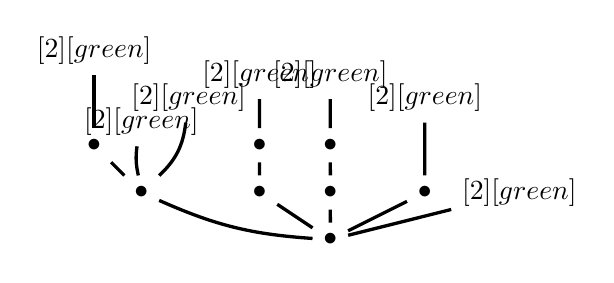
\begin{tikzpicture}[very thick, scale=0.3]
\node (foot) at (10,0) {$\bullet$};
\node (N1) at (2,2) {$\bullet$};
\node (N2) at (10,2) {$\bullet$};
\node (N22) at (7,2) {$\bullet$};
\node (N3) at (14,2) {$\bullet$};
\node (N4) at (18,2) {$\Smiley[2][green]$};
\node (N5) at (0,4) {$\bullet$};
\node (N6) at (2,5) {$\Smiley[2][green]$};
\node (N7) at (4,6) {$\Smiley[2][green]$};
\node (N88) at (7,4) {$\bullet$};
\node (N8) at (10,4) {$\bullet$};
\node (N9) at (14,6) {$\Smiley[2][green]$};
\node (N10) at (0,8) {$\Smiley[2][green]$};
\node (N11) at (10,7) {$\Smiley[2][green]$};
\node (N111) at (7,7) {$\Smiley[2][green]$};
\draw (foot) to [bend left=10] (N1);
\draw (foot) -- (N2);
\draw (foot) -- (N22);
\draw (foot) -- (N3);
\draw (foot) -- (N4);
\draw (N1) to  (N5);
\draw (N1) to   [bend left=10] (N6);
\draw (N1) to   [bend right=20] (N7);
\draw (N2) to  (N8);
\draw (N22) to  (N88);
\draw (N8) to  (N11);
\draw (N88) to  (N111);
\draw (N3) to  (N9);
\draw (N5) to  (N10);
\end{tikzpicture}
\caption{The hydra $\iota(\omega^{\omega+2}+\omega^\omega \times 2 + \omega + 1$) \label{fig:iota-example}}

\end{figure}


The following lemma (proved in ~\href{../theories/html/hydras.Hydra.O2H.html}{Hydra.O2H.v}) maps  canonical sequences to rounds of hydra battles.


\label{lemma:canonS-iota}

\input{movies/snippets/O2H/canonSIota}

The next step of our development extends this relationship to
the order $<$ on $[0,\epsilon_0)$ on one side, and hydra battles on the other side.

\input{movies/snippets/O2H/pathToRoundPlus}

As a corollary, we are now able to transform any inequality $\beta<\alpha<\epsilon_0$ into a (free) battle.

\input{movies/snippets/O2H/LTToRoundPlus}


\section{A  proof of impossibility}
\label{sect:impossibility-free}

We now have  the tools for proving that  there exists no variant bounded by some $\mu<\epsilon_0$ for proving the termination   of all battles. The proof we are going to show is a proof by contradiction. It  can
 be considered as a generalization of the
proofs described in  sections~\vref{omega-case} and \vref{omega2-case}.



In the module
\href{../theories/html/hydras.Hydra.Epsilon0_Needed_Generic.html}{Hydra.Epsilon0\_Needed\_Generic}, we assume there exists some variant $m$ bounded by some ordinal $\mu<\epsilon_0$. This part of the development is parameterized by some class $B$ of battles, which will be instantiated later to \texttt{free} or \texttt{standard}.

\vspace{4pt}
\noindent
From~\href{../theories/html/hydras.Hydra.~Hydra_Definitions.html}{Hydra.Hydra\_Definitions}:

\input{movies/snippets/Hydra_Definitions/BoundedVariant}

Let us assume there exists such a variant:

\input{movies/snippets/Epsilon0_Needed_Generic/theContext}

\label{remark:m-decrease}
\begin{remark}
  The hypothesis \texttt{m\_decrease} is not provable  in general, but is satisfied by
the  \texttt{free} and \texttt{standard} kinds of battles. This trick allows to 
``factorize'' our proofs  of impossibility.
\end{remark}

\index{maths}{Transfinite induction}

First, we prove that $m(\iota(\alpha))$ is always greater than or equal to $\alpha$, by  transfinite induction over $\alpha$.


\input{movies/snippets/Epsilon0_Needed_Generic/mGe0}

\begin{itemize}
\item If $\alpha=0$, the inequality trivially holds
\item If $\alpha$ is the successor of  some ordinal $\beta$, the inequality $\beta \leq m(\iota(\beta))$ holds (by induction hypothesis). But the hydra $\iota(\alpha)$ is transformed in one round into 
$\iota(\beta)$, thus $m(\iota(\beta))<m(\iota(\alpha))$. Hence $\beta<m(\iota(\alpha))$, which implies $\alpha \leq m(\iota(\alpha))$
\item If $\alpha$ is a limit ordinal, then $\alpha$ is the least upper bound of the set
of all  the $\canonseq{\alpha}{i}$.  Thus, we have just to prove that $\canonseq{\alpha}{i}< m(\iota(\alpha))$ for any $i$. 
\begin{itemize}
\item Let $i$ be some natural number.
By the induction hypothesis, we have $\canonseq{\alpha}{i} \leq m(\iota(\canonseq{\alpha}{i}))$. But the hydra $\iota(\alpha)$ is transformed into $\iota(\canonseq{\alpha}{i})$ in one round, thus $m(\iota(\canonseq{\alpha}{i})) < m(\iota(\alpha))$, by our hypothesis \texttt{m\_decrease}.
\end{itemize}
\end{itemize}

Please note that the impossibility proofs of 
sections~\vref{omega-case} and \vref{omega2-case} contain a similar lemma, also called \texttt{m\_ge}.
We are now able to build a counter-example.
\label{sect:mge-generic}

\input{movies/snippets/Epsilon0_Needed_Generic/mGeGeneric}

The (big) rest of the proof is dedicated to prove formally the converse inequality 
\texttt{m small\_h t1< m big\_h}. 

\subsection{The case of free battles}
\label{sec:free-battles-case}
Let us now consider that $B$ is instantiated to \texttt{free} (which means that we are considering proofs of termination of \emph{all} battles). The following lemmas are proved in Module~\href{../theories/html/hydras.Hydra.Epsilon0_Needed_Free.html}{Hydra.Epsilon0\_Needed\_Free}.
The case $B=\texttt{standard}$ is studied in section~\vref{std-case}.


\input{movies/snippets/Epsilon0_Needed_Free/theContext}


\begin{enumerate}
\item The following lemma is an application of \texttt{m\_ge\_generic}, since \texttt{free}
satisfies trivially the hypothesis \texttt{m\_decrease} (see page~\pageref{remark:m-decrease}).

\inputsnippets{Epsilon0_Needed_Free/mGe}


\item From the hypothesis \texttt{Hy}, we have \texttt{m big\_h t1< mu}
\item By Lemma \texttt{LT\_to\_round\_plus}, we get a (free) battle from
\texttt{big\_h = iota mu} to \texttt{small\_h = iota (m big\_h)}.

\input{movies/snippets/Epsilon0_Needed_Free/bigToSmall}


\item From the hypotheses on $m$, we infer:
\input{movies/snippets/Epsilon0_Needed_Free/mLt}

\item From lemmas \texttt{m\_ge} and \texttt{m\_lt}, and the irreflexivity of $<$, we get a contradiction. 
\input{movies/snippets/Epsilon0_Needed_Free/ImpossibilityFree}

\end{enumerate}

We have now proved there exists no bounded variant for the class of free battles.


\input{movies/snippets/Epsilon0_Needed_Free/CheckDemo}


\paragraph*{\gaiasign} Please look at the \gaia version of this theorem in Sect.~\vref{sect:impossibility-gaia-version}.
\index{gaiabridge}{Impossibility theorems}
\section{The case of standard battles}
\label{sec:standard-intro}\label{std-case}
One may wonder if our theorem holds also in the framework of standard battles. Unfortunately, its proof relies on the lemma \texttt{LT\_to\_round\_plus} of
Module~\href{../theories/html/hydras.Hydra.O2H.html}{Hydra.O2H}.

\input{movies/snippets/O2H/LTToRoundPlus}

This lemma builds a battle out of any inequality $\beta<\alpha$. 
It is a straightforward application of \texttt{LT\_path\_to} of
Module~\href{../theories/html/hydras.Epsilon0.Paths.html}{Epsilon0.Paths}:

\input{movies/snippets/Paths/LTPathTo}

The sequence $s$, used to build the sequence of replication factors of the battle, depends on 
$\alpha$ and $\beta$, so we cannot be sure that the generated battle is a genuine standard battle.


The solution to this issue comes  once again from Ketonen and Solovay's article~\cite{KS81}. Instead of considering plain paths, i.e. sequences 
$\alpha_0=\alpha,\alpha_1,\dots,\alpha_k=\beta$ where $\alpha_{j+1}$ is equal
to $\canonseq{\alpha_j}{i_j}$ where $i_j$ is \emph{any} natural number, 
we consider various constraints on these sequences.
In particular, a path is called \emph{standard} if $i_{j+1} = i_j + 1$ for every $j<k$.
It  corresponds to a ``segment'' of some standard battles. 
Please note that the vocabulary on paths is ours, but all the concepts come really from~\cite{KS81}.

In \coq{}, standard paths can be defined as follows.

\vspace{4pt}

\emph{From
Module~\href{../theories/html/hydras.Epsilon0.Paths.html}{Epsilon0.Paths}}

\input{movies/snippets/Paths/standardPathR}

In the mathematical text and figures, we shall use the notation 
$\alpha \xrightarrow[i,j]{}\beta$ for the proposition 
(\texttt{standard\_path $i$ $\alpha$ $j$ $\beta$}).
In~\cite{KS81} the notation is
$\alpha \xrightarrow[i]{*}\beta$
for 
the proposition  $\exists j, i<j \wedge \alpha \xrightarrow[i,j]{} \beta$.



Our goal is now  to transform any inequality $\beta<\alpha<\epsilon_0$ into a standard path $\alpha \xrightarrow[i,j]{} \beta$ for some $i$ and $j$, which corresponds to a standard battle
from $\iota(\alpha)$ (at time $i$)  to $\iota(\beta)$
(at time $j$) .
Following~\cite{KS81}, we proceed in two stages:
\begin{enumerate}
\item we simulate plain (free) paths from $\alpha$ to $\beta$ with
paths made of steps $(\gamma,\canonseq{\gamma}{n})$, \emph{with the same $n$ all along the path}.
\item we simulate any such path by a standard path.
\end{enumerate}



\subsection{Paths with a constant index}

First of all, paths with a constant index 
enjoy nice properties. They are defined as paths where all the $i_j$ are equal to the same natural number $i$, for some $i>0$. 


Like in~\cite{KS81}, we shall use the notation $\alpha \xrightarrow[i]{} \beta$ for denoting such a path, also called an $i$-path.

\input{movies/snippets/Paths/constPathDef}

% Paths with a given index can be effectively computed.
% Given $i$, $\alpha$ and $l$, the following function returns the ordinal $\beta$ such that there exists a path 
% $\alpha \xrightarrow [i+1] {} \beta$ of length $l$. 

% \begin{Coqsrc}
% Fixpoint const_funS (i:nat)(alpha : T1)(l:nat):  T1  :=
%   match l
%   with
%   | 0 => alpha
%   | S m => const_funS i (canonS i alpha) m
%   end.
% \end{Coqsrc}

% The following computations show  applications of \texttt{constS\_fun} to the 
% ordinal $\omega^\omega$, with various values of $i$ and $l$.

% \begin{Coqsrc}
% Compute  (const_funS 2 (omega ^omega)  55).
% \end{Coqsrc}

% \begin{Coqanswer}
%   = zero
%      : T1 
% \end{Coqanswer}

% \begin{Coqsrc}
% Compute pp (const_funS 2 (omega ^omega) 15).
% \end{Coqsrc}

%   \begin{Coqanswer}
%  = (omega ^ 2 * 2)%pT1
%      : ppT1   
%   \end{Coqanswer}


% \begin{Coqsrc}
% Compute pp (const_funS 4 (omega^omega)  100).
% \end{Coqsrc}

% \begin{Coqanswer}
% = (omega ^ 4 * 4 + omega ^ 3 * 4 + omega ^ 2 + omega * 4 + 4)%pT1
%      : ppT1
% \end{Coqanswer}


A most interesting property of $i$-paths is that we can ``upgrade'' their index, as stated by K.\&S.'s Corollary 12.

\index{maths}{Transfinite induction}

\vspace{4pt}
\noindent
\emph{From
  Module~\href{../theories/html/hydras.Epsilon0.Paths.html}{Epsilon0.Paths}}

\input{movies/snippets/Paths/Cor12}


We  also use a version of \texttt{Cor12} with large inequalities.

\input{movies/snippets/Paths/Cor121}


\texttt{Cor12} is a consequence of the following theorem (numbered \texttt{2.4} in Ketonen and Solovay's article), proven by transfinite induction on $\alpha$.

\input{movies/snippets/Paths/KSThm24}

\vspace{4pt}

\subsubsection{Sketch of proof of \texttt{Cor12}}
\index{maths}{Transfinite induction}

\texttt{Cor12} is also proved by transfinite induction on $\alpha$.  Let us give  a sketch of its proof \footnote{This proof sketch is a slight simplification of the formal proof script:
  The strictly positive indexes $i$ and $n$ stand for the
  terms \texttt{(S i)} and \texttt{(S n)}. We do not explicit  the (simpler) case where the considered path is made of only one step.}

Let us consider a path $\alpha \xrightarrow [i]{} \beta$ $(i>0)$. Its first step is
the pair $(\alpha,\canonseq{\alpha}{i})$, We have $\canonseq{\alpha}{i}<\alpha$ and
$\canonseq{\alpha}{i} \xrightarrow [i]{} \beta$. 
Let $n$ be any natural number such that $n>i$.
By the induction hypothesis, there exists a path $\canonseq{\alpha}{n} \xrightarrow[i]{} \beta$.
\begin{itemize}
\item  If $\alpha$ is a successor ordinal $\gamma+1$, then $\canonseq{\alpha}{n} =
\canonseq{\alpha}{i}=\gamma$. Thus we have a path 
$\alpha  \xrightarrow [n]{}  \gamma \xrightarrow [n]{} \beta$
\item If $\alpha$ is a limit ordinal, we apply Theorem \texttt{KS\_thm\_2\_4} (see above).

%   \begin{theorem}
% Let $\lambda$ be a limit ordinal, then for any pair of indices $0<i<j$, there is a path $\canonseq{\lambda}{j} \xrightarrow[1]{} \canonseq{\lambda}{i}$.    
%   \end{theorem}


  

The proof of the limit case, is decomposed into a sequence
of path constructions leading to $\alpha \xrightarrow[n]{} \beta$.

 \begin{enumerate}
 \item $\alpha \xrightarrow[n]{} \canonseq{\alpha}{n}$ (single step path)
 \item $\canonseq{\alpha}{n} \xrightarrow[1]{} \canonseq{\alpha}{i}$ (by \texttt{Theorem\_2\_4}),
\item $\canonseq{\alpha}{n} \xrightarrow[n]{} \canonseq{\alpha}{i}$ (applying the induction hypothesis to the preceding path);
\item $\canonseq{\alpha}{i} \xrightarrow[n]{} \beta$ (applying the induction hypothesis)
\item $\alpha \xrightarrow[n]{} \beta$ (by composition of 1, 3, and 4).


 \end{enumerate}


\end{itemize}


\begin{remark}
 \texttt{Cor12} ``casts'' $i$-paths into $n$-paths for any $n>i$.
But the obtained $n$-path can be much longer than the original $i$-path.
The following exercise will give an idea of this increase. 
\end{remark}

\index{hydras}{Exercises}
\begin{exercise}
  Prove that  the length of the $i+1$-path from
  $\omega^\omega$ to $\omega^i$ is $1 + (i+1)^{(i+1)}$, for any $i$. Note that the $i$-path from
  $\omega^\omega$ to $\omega^i$ is only one step long.
 \end{exercise}




Why is \texttt{Cor12} so useful? 
Let us  consider two ordinals  $\beta<\alpha<\epsilon_0$. By induction on $\alpha$,
we decompose any inequality $\beta<\alpha$ into $\beta < \canonseq{\alpha}{i}< \alpha$, where $i$ is some natural number. Applying corollary \texttt{Cor12'} we build a $n$-path from $\beta$ to $\alpha$,
where $n$ is the maximum of the indices $i$ met in the induction.

 Lemma 1, Section 2.6 of~\cite{KS81} is naturally expressed in terms of \coq's
\verb@sig@ construct.

\label{lemma:L-2_6-1}
%\index{coq}{Sigma types}

\input{movies/snippets/Paths/Lemma261}


Intuitively, Lemma~\texttt{2\_6\_1}  shows that if $\beta<\alpha<\epsilon_0$, then there exists  a battle from $\iota(\alpha)$ to $\iota(\beta)$ where the replication factor is constant, although large enough. 






 \paragraph*{\gaiasign}
 Corollary \texttt{Cor12} and Lemma \texttt{Lemma2\_6\_1} are also available in
\href{../theories/html/gaia_hydras.GPaths.html}{gaia\_hydras.GPaths} 
(please see Sect.~\vref{sect:gpath}).

\subsection{Casting paths with a constant index into a standard path}


The article~\cite{KS81} contains 
the following lemma, which allows us to simulate $i$-paths by $[i+1,j]$-paths, where $j$ is large enough.

\input{movies/snippets/Paths/constantToStandard}

\subsubsection{Sketch of proof of \texttt{constant\_to\_standard\_path}}

Our proof follows the proof by Ketonen and Solovay, including its organization as a sequence of lemma.  Since it is a non-trivial proof, we will comment its main steps below   (see Figure~\vref{fig:belle-preuve-1} to Figure~\vref{fig:fin-belle-preuve}).

\subsubsection*{Preliminaries}


Please note that, given an ordinal $\alpha:\texttt{T1}$, and two natural numbers $i$ and $l$, there exists at most a standard path $\alpha \xrightarrow [i,i+l]{*} \beta$.
The following function computes $\beta$ from $\alpha$, $i$ and $l$.

\input{movies/snippets/Paths/standardGnaw}



\index{maths}{Transfinite induction}

By transfinite induction over  $\alpha$, we prove that the ordinal $0$ is reachable from any ordinal $\alpha<\epsilon_0$ by some standard path.

\input{movies/snippets/Paths/standardPathToZero}


\paragraph*{}
Now, let us consider two ordinals  $\beta<\alpha<\epsilon_0$.  Let $p$  be some $(n+1)$-path from $\alpha$ to $\beta$.

\input{movies/snippets/Paths/ConstantToStandardProof}


Applying \texttt{standard\_path\_to\_zero}, $0$ is reachable from $\alpha$ by some standard path.

\begin{figure}[h]
  \centering
 
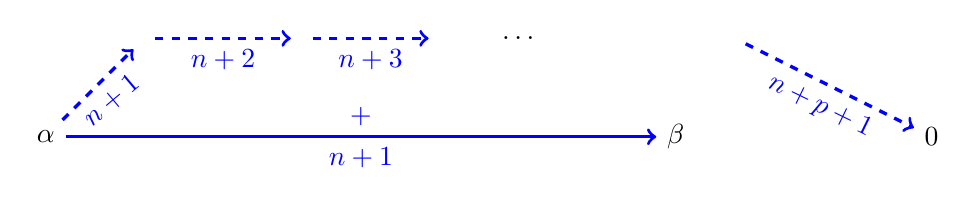
\begin{tikzpicture}[very thick, scale=0.25]
\node (alpha) at (0,0) {$\alpha$};
    \node (beta) at (32, 0){$\beta$};
  

  \draw[->, very thick,blue] (alpha)-- node [below]{$n+1$} node [above] {$+$} (beta);

  \node (alpha1) at (5,5) {};
  \node (alpha2) at (13,5) {};
    \node (alpha3) at (20,5) {};
  \node (alphalast) at (35,5) {};
  \node (zero) at (45,0) {$0$};
  \draw [->, dashed,very thick,blue] (alpha)-- node [below, rotate=40]{$n+1$}  (alpha1);
  \draw [->, dashed,very thick,blue] (alpha1)-- node [below]{$n+2$}  (alpha2);
   \draw [->, dashed,very thick,blue] (alpha2)-- node [below]{$n+3$}  (alpha3);
  
  \node (dots) at (24,5) {$\dots$};
  \draw [->, dashed, very thick,blue] (alphalast)-- node [below, rotate=-26]{$n+p+1$}  (zero);

\end{tikzpicture}
\caption{A nice proof (1)}
  \label{fig:belle-preuve-1}
\end{figure}


\paragraph*{}




Since comparison on \texttt{T1} is decidable, one can compute the last step $\gamma$ of the standard path from $(\alpha,n+1)$  such that $\beta\leq \gamma$.
Let $l$ be the length of the path from $\alpha$ to $\gamma$.  
This step of the proof is illustrated in figure~\vref{fig:belle-preuve-2} \footnote{Please note that in these figures, smaller ordinals are represented on the right side!}.



\begin{figure}[h]
  \centering
 

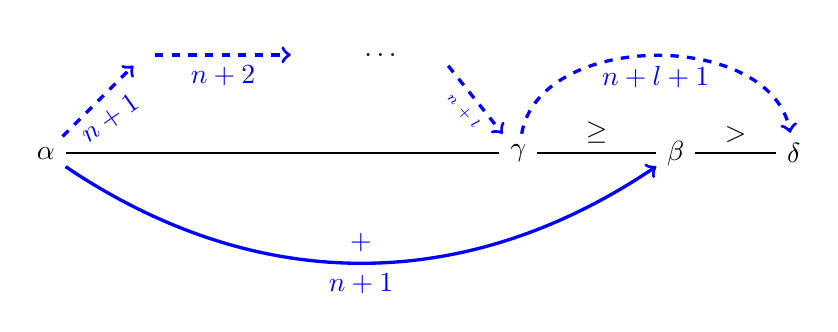
\begin{tikzpicture}[very thick, scale=0.25]
\node (alpha) at (0,0) {$\alpha$};
    \node (beta) at (32, 0){$\beta$};
  



  \node (alpha1) at (5,5) {};
  \node (alpha2) at (13,5) {};
  \node (dots) at (17,5) {$\ldots$};
    \node (alpha3) at (20,5) {};
    \node (gamma) at (24,0) {$\gamma$};
    \node (delta) at (38,0) {$\delta$};
    \draw [->, dashed,very thick,blue] (alpha)-- node [below,rotate=35]{$n+1$}  (alpha1);
  \draw [->, dashed,very thick,blue] (alpha1)-- node [below]{$n+2$}  (alpha2);
   \draw [->, dashed,very thick,blue] (alpha3)-- node [below,rotate = -48]{\tiny $n+l$}  (gamma);
   \draw  [->, dashed, blue] (gamma) to    [bend left=80] node [below]{$n+l+1$} (delta);
   \draw[->, very thick,blue] (alpha) to [bend right=34] node [below]{$n+1$} node [above] {$+$} (beta);
   \draw[thick] (alpha)--  (gamma);
   \draw[thick] (gamma)--  node [above] {$\geq$} (beta);
    \draw[thick] (beta)--  node [above] {$>$} (delta);
\end{tikzpicture}

\caption{A nice proof (2)}
  \label{fig:belle-preuve-2}
\end{figure}

\paragraph*{}

\begin{itemize}
\item If $\beta=\gamma$, it's OK! We have got a standard path
from  
$\alpha$ to $\beta$ with successive indices  $n+1, n+2, \dots, n+l+1$

\item Otherwise,  $\beta < \gamma$.  Let us consider  $\delta=\canonseq{\gamma}{n+l+1}$.
By applying several times lemma \texttt{Cor12},  one converts  every path of Fig~\ref{fig:belle-preuve-2} into
 a $n+l+1$-path  (see figure~\ref{fig:belle-preuve-3}).


But $\gamma$ is on the $n+l+1$-path from $\alpha$ to $\beta$.
As shown by figure~\vref{fig:fin-belle-preuve}, the ordinal $\delta$, reachable from
$\gamma$ in one single step,  must be greater than or equal to $\beta$, which contradicts our  hypothesis $\beta < \gamma$.


\begin{figure}[h]
  \centering
  
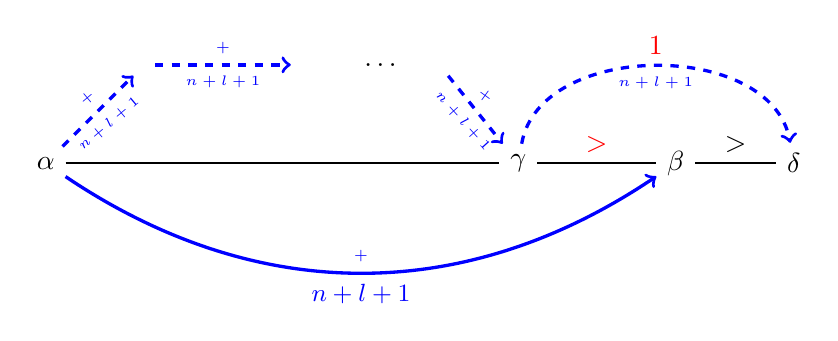
\begin{tikzpicture}[very thick, scale=0.25]
\node (alpha) at (0,0) {$\alpha$};
    \node (beta) at (32, 0){$\beta$};
    \node (alpha1) at (5,5) {};
  \node (alpha2) at (13,5) {};
  \node (dots) at (17,5) {$\ldots$};
    \node (alpha3) at (20,5) {};
    \node (gamma) at (24,0) {$\gamma$};
    \node (delta) at (38,0) {$\delta$};
     \draw [->, dashed,very thick,blue] (alpha)-- node [below, rotate = 40] {\tiny $n+l+1$}  node [above, rotate = 40]{\tiny $+$}  (alpha1);
  \draw [->, dashed,very thick,blue] (alpha1)-- node [below]{\tiny $n+l+1$} node [above]{\tiny $+$} (alpha2);
   \draw [->, dashed,very thick,blue] (alpha3)-- node [below, rotate = -48]{\tiny $n+l+1$} node [above, rotate = -36]{\tiny $+$}  (gamma);
   \draw  [->, dashed, blue] (gamma) to    [bend left=80] node [below]{\tiny $n+l+1$} node [above]{\color{red} $1$} (delta);
   \draw[->, very thick,blue] (alpha) to [bend right=34] node [below]{\small $n+l+1$} node [above] {\tiny $+$} (beta);
    \draw[thick] (gamma)--   node [above]{\color{red} $>$}(beta);
   \draw[thick] (alpha)--  (gamma);
  
    \draw[thick] (beta)--  node [above] {$>$} (delta);

  
  
\end{tikzpicture}

\caption{A nice proof (3)}
  \label{fig:belle-preuve-3}
\end{figure}


\begin{figure}[h]
  \centering
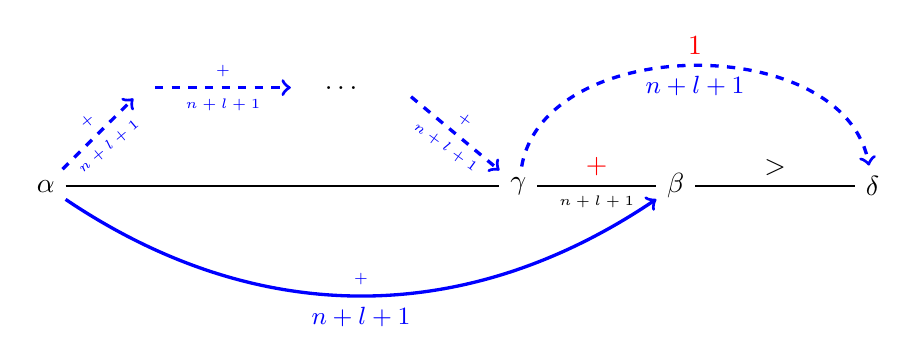
\begin{tikzpicture}[very thick, scale=0.25]
\node (alpha) at (0,0) {$\alpha$};
    \node (beta) at (32, 0){$\beta$};
  
  \node (alpha1) at (5,5) {};
  \node (alpha2) at (13,5) {};
  \node (dots) at (15,5) {$\ldots$};
    \node (alpha3) at (18,5) {};
    \node (gamma) at (24,0) {$\gamma$};
    \node (delta) at (42,0) {$\delta$};
    \draw [->, dashed,very thick,blue] (alpha)-- node [below, rotate = 40] {\tiny $n+l+1$}  node [above, rotate = 40]{\tiny $+$}  (alpha1);
  \draw [->, dashed,very thick,blue] (alpha1)-- node [below]{\tiny $n+l+1$} node [above]{\tiny $+$} (alpha2);
   \draw [->, dashed,very thick,blue] (alpha3)-- node [below, rotate = -36]{\tiny $n+l+1$} node [above, rotate = -36]{\tiny $+$}  (gamma);
   \draw  [->, dashed, blue] (gamma) to    [bend left=80] node [below]{\small $n+l+1$} node [above]{\color{red} $1$} (delta);
   \draw[->, very thick,blue] (alpha) to [bend right=34] node [below]{\small $n+l+1$} node [above] {\tiny $+$} (beta);
   \draw[thick] (alpha)--  (gamma);
  
    \draw[thick] (gamma)--  node [below]{\tiny $n+l+1$} node [above]{\color{red} $+$}(beta);
    \draw[thick] (beta)--  node [above] {$>$} (delta);

\end{tikzpicture}

\caption{A nice proof (4)}
  \label{fig:fin-belle-preuve}
\end{figure}


\end{itemize}
 The only possible case is  thus $\beta=\gamma$, so we have got a standard path  from $\alpha$ to $\beta$.

 \input{movies/snippets/Paths/constantToStandard0}
 \input{movies/snippets/Paths/constantToStandardz}
 


Here is the full statement of the conversion from constant to standard paths.

\input{movies/snippets/Paths/constantToStandardPath}


Applying \texttt{Lemma2\_6\_1} and \texttt{constant\_to\_standard\_path}, we get the following corollary.

\input{movies/snippets/Paths/LTToStandardPath}


\subsection{Back to hydras}
\label{sec:standard-battles-cases}
We are now able to complete our proof that there exists no bounded variant for proving the termination of standard hydra battles. This proof can
be consulted in the module 
\href{../theories/html/hydras.Hydra.Epsilon0_Needed_Std.html}{Hydra.Epsilon0\_Needed\_Std}.
Please note that it has the same global structure as in section~\ref{sec:free-battles-case} 

Applying the  lemmas  \texttt{Lemma2\_6\_1} of the module 
\href{../theories/html/hydras.Epsilon0.Paths.html\#Lemma2_6_1}%
{Epsilon0.pathS}   and 
\href{../theories/html/hydras.Epsilon0.Paths.html\#constant_to_standard_path}%
{\texttt{constant\_to\_standard\_path}},
we can convert any inequality $\beta<\alpha<\epsilon_0$ into a standard path from
$\alpha$ to  $\beta$, then into a fragment of a standard battle from 
$\iota(\alpha)$ to $\iota(\beta)$, hence the inequality $m(\iota(\beta))<m(\iota(\alpha))$.


\vspace{4pt}
\emph{From Module~\href{../theories/html/hydras.Hydra.Epsilon0_Needed_Std.html\#LT_to_standard_battle}{Hydra.Epsilon0\_Needed\_Std}}

\input{movies/snippets/Epsilon0_Needed_Std/LTToStandardBattle}


Now, please consider the following context:

\input{movies/snippets/Epsilon0_Needed_Std/theContext}

In the same way as for free battles, we import a large inequality 
from 
the module \href{../theories/html/hydras.Hydra.Epsilon0_Needed_Generic.html}{Epsilon0\_Needed\_Generic}.
(see Sect.~\vref{sect:mge-generic}).

\input{movies/snippets/Epsilon0_Needed_Std/mGe}



\paragraph*{} If remains to prove the following strict inequality, in order to have a contradiction.

\input{movies/snippets/Epsilon0_Needed_Std/mLt}


\paragraph*{Sketch of proof:} Let us recall that $\texttt{big\_h} = \iota(\mu)$
 and $\texttt{small\_h} = \iota (m (\texttt{big\_h}))$.

Since $m(\texttt{big\_h})< \mu$, there exists a standard path from $\mu$ to
$m(\texttt{big\_h})$, hence a   standard battle from $\iota(\mu)$  to
$\iota(m(\texttt{big\_h}))$,  i.e. from \texttt{big\_h} to \texttt{small\_h}.

Since $m$ is assumed to be a variant for standard battles, we get the inequality  $m(\texttt{small\_h}) < m(\texttt{big\_h})$.


\input{movies/snippets/Epsilon0_Needed_Std/endOfProof}

\paragraph*{\gaiasign} Please look at the \gaia version of this theorem in Sect.~\vref{sect:impossibility-gaia-version}.
\index{gaiabridge}{Impossibility theorems}



\subsection{Remarks}

We are grateful to 
 J. Ketonen and R. Solovay  for the high quality of their explanations and proof details.
Our proof follows tightly the sequence of lemmas in their article, with a focus on 
constructive aspects.
Roughly speaking, our implementation \emph{builds}, out of a hypothetical
  variant $m$, bounded by some ordinal $\mu<\epsilon_0$, a hydra \texttt{big\_h} which verifies the impossible inequality  $m(\texttt{big\_h})< m(\texttt{big\_h})$.



On may ask whether the preceding results are too restrictive, since they 
refer to a particular data type \texttt{T1}.
In fact, our representation of ordinals strictly less than 
 $\epsilon_0$ is faithful to their mathematical definition, at least 
Kurt Schütte's~\cite{schutte}, as proved in Chapter~\vref{chap:schutte}.
(please see also the module
\href{../theories/html/hydras.Schutte.Correctness_E0.html}{hydras.Schutte.Correctness\_E0}).

Thus, we can infer that our theorems can be applied to any well order.

\index{hydras}{Projects}
\begin{project}
Study a possible modification of the definition of a variant  (for  standard battles).

\begin{itemize}
\item The variant is assumed to be strictly decreasing \emph{on configurations 
reachable from some initial configuration where the replication factor is equal to $0$}
\item The variant may depend on the number of the current round.
\end{itemize}

In other words, its type should be \texttt{nat -> Hydra -> T1}, and it must 
verify the inequality $m\, (S\,i)\, h' < m\,i\, h$ whenever the configuration 
$(i,h)$ is reachable from some initial configuration $(0,h_0)$
and \texttt{h} is transformed into \texttt{h'} in the considered round.
Can we still prove the theorems of section~\ref{std-case} with this new definition?

\end{project}
